% Options for packages loaded elsewhere
\PassOptionsToPackage{unicode}{hyperref}
\PassOptionsToPackage{hyphens}{url}
%
\documentclass[
]{article}
\usepackage{amsmath,amssymb}
\usepackage{lmodern}
\usepackage{iftex}
\ifPDFTeX
  \usepackage[T1]{fontenc}
  \usepackage[utf8]{inputenc}
  \usepackage{textcomp} % provide euro and other symbols
\else % if luatex or xetex
       %%% MODIFIED: unicode-math conflics with expex; mathspects conflicts with glossaries/leipzig
  \usepackage{fontspec} % \usepackage{unicode-math}
  \defaultfontfeatures{Scale=MatchLowercase}
  \defaultfontfeatures[\rmfamily]{Ligatures=TeX,Scale=1}
  \setmainfont[]{DejaVu Sans}
\fi
% Use upquote if available, for straight quotes in verbatim environments
\IfFileExists{upquote.sty}{\usepackage{upquote}}{}
\IfFileExists{microtype.sty}{% use microtype if available
  \usepackage[]{microtype}
  \UseMicrotypeSet[protrusion]{basicmath} % disable protrusion for tt fonts
}{}
\makeatletter
\@ifundefined{KOMAClassName}{% if non-KOMA class
  \IfFileExists{parskip.sty}{%
    \usepackage{parskip}
  }{% else
    \setlength{\parindent}{0pt}
    \setlength{\parskip}{6pt plus 2pt minus 1pt}}
}{% if KOMA class
  \KOMAoptions{parskip=half}}
\makeatother
\usepackage{xcolor}
\IfFileExists{xurl.sty}{\usepackage{xurl}}{} % add URL line breaks if available
\IfFileExists{bookmark.sty}{\usepackage{bookmark}}{\usepackage{hyperref}}
\hypersetup{
  pdftitle={QML - Formative Assessment 1},
  pdfauthor={YOUR EXAM NUMBER},
  hidelinks,
  pdfcreator={LaTeX via pandoc}}
\urlstyle{same} % disable monospaced font for URLs
\usepackage[margin=1in]{geometry}
\usepackage{color}
\usepackage{fancyvrb}
\newcommand{\VerbBar}{|}
\newcommand{\VERB}{\Verb[commandchars=\\\{\}]}
\DefineVerbatimEnvironment{Highlighting}{Verbatim}{commandchars=\\\{\}}
% Add ',fontsize=\small' for more characters per line
\usepackage{framed}
\definecolor{shadecolor}{RGB}{248,248,248}
\newenvironment{Shaded}{\begin{snugshade}}{\end{snugshade}}
\newcommand{\AlertTok}[1]{\textcolor[rgb]{0.94,0.16,0.16}{#1}}
\newcommand{\AnnotationTok}[1]{\textcolor[rgb]{0.56,0.35,0.01}{\textbf{\textit{#1}}}}
\newcommand{\AttributeTok}[1]{\textcolor[rgb]{0.13,0.29,0.53}{#1}}
\newcommand{\BaseNTok}[1]{\textcolor[rgb]{0.00,0.00,0.81}{#1}}
\newcommand{\BuiltInTok}[1]{#1}
\newcommand{\CharTok}[1]{\textcolor[rgb]{0.31,0.60,0.02}{#1}}
\newcommand{\CommentTok}[1]{\textcolor[rgb]{0.56,0.35,0.01}{\textit{#1}}}
\newcommand{\CommentVarTok}[1]{\textcolor[rgb]{0.56,0.35,0.01}{\textbf{\textit{#1}}}}
\newcommand{\ConstantTok}[1]{\textcolor[rgb]{0.56,0.35,0.01}{#1}}
\newcommand{\ControlFlowTok}[1]{\textcolor[rgb]{0.13,0.29,0.53}{\textbf{#1}}}
\newcommand{\DataTypeTok}[1]{\textcolor[rgb]{0.13,0.29,0.53}{#1}}
\newcommand{\DecValTok}[1]{\textcolor[rgb]{0.00,0.00,0.81}{#1}}
\newcommand{\DocumentationTok}[1]{\textcolor[rgb]{0.56,0.35,0.01}{\textbf{\textit{#1}}}}
\newcommand{\ErrorTok}[1]{\textcolor[rgb]{0.64,0.00,0.00}{\textbf{#1}}}
\newcommand{\ExtensionTok}[1]{#1}
\newcommand{\FloatTok}[1]{\textcolor[rgb]{0.00,0.00,0.81}{#1}}
\newcommand{\FunctionTok}[1]{\textcolor[rgb]{0.13,0.29,0.53}{\textbf{#1}}}
\newcommand{\ImportTok}[1]{#1}
\newcommand{\InformationTok}[1]{\textcolor[rgb]{0.56,0.35,0.01}{\textbf{\textit{#1}}}}
\newcommand{\KeywordTok}[1]{\textcolor[rgb]{0.13,0.29,0.53}{\textbf{#1}}}
\newcommand{\NormalTok}[1]{#1}
\newcommand{\OperatorTok}[1]{\textcolor[rgb]{0.81,0.36,0.00}{\textbf{#1}}}
\newcommand{\OtherTok}[1]{\textcolor[rgb]{0.56,0.35,0.01}{#1}}
\newcommand{\PreprocessorTok}[1]{\textcolor[rgb]{0.56,0.35,0.01}{\textit{#1}}}
\newcommand{\RegionMarkerTok}[1]{#1}
\newcommand{\SpecialCharTok}[1]{\textcolor[rgb]{0.81,0.36,0.00}{\textbf{#1}}}
\newcommand{\SpecialStringTok}[1]{\textcolor[rgb]{0.31,0.60,0.02}{#1}}
\newcommand{\StringTok}[1]{\textcolor[rgb]{0.31,0.60,0.02}{#1}}
\newcommand{\VariableTok}[1]{\textcolor[rgb]{0.00,0.00,0.00}{#1}}
\newcommand{\VerbatimStringTok}[1]{\textcolor[rgb]{0.31,0.60,0.02}{#1}}
\newcommand{\WarningTok}[1]{\textcolor[rgb]{0.56,0.35,0.01}{\textbf{\textit{#1}}}}
\usepackage{longtable,booktabs,array}
\usepackage{calc} % for calculating minipage widths
% Correct order of tables after \paragraph or \subparagraph
\usepackage{etoolbox}
\makeatletter
\patchcmd\longtable{\par}{\if@noskipsec\mbox{}\fi\par}{}{}
\makeatother
% Allow footnotes in longtable head/foot
\IfFileExists{footnotehyper.sty}{\usepackage{footnotehyper}}{\usepackage{footnote}}
\makesavenoteenv{longtable}
\usepackage{graphicx}
\makeatletter
\def\maxwidth{\ifdim\Gin@nat@width>\linewidth\linewidth\else\Gin@nat@width\fi}
\def\maxheight{\ifdim\Gin@nat@height>\textheight\textheight\else\Gin@nat@height\fi}
\makeatother
% Scale images if necessary, so that they will not overflow the page
% margins by default, and it is still possible to overwrite the defaults
% using explicit options in \includegraphics[width, height, ...]{}
\setkeys{Gin}{width=\maxwidth,height=\maxheight,keepaspectratio}
% Set default figure placement to htbp
\makeatletter
\def\fps@figure{htbp}
\makeatother
\setlength{\emergencystretch}{3em} % prevent overfull lines
\providecommand{\tightlist}{%
  \setlength{\itemsep}{0pt}\setlength{\parskip}{0pt}}
\setcounter{secnumdepth}{5}
\ifLuaTeX
  \usepackage{selnolig}  % disable illegal ligatures
\fi

\title{QML - Formative Assessment 1}
\author{YOUR EXAM NUMBER}
\date{2023-09-08}

\begin{document}
\maketitle

\section{Instructions}\label{instructions}

\textbf{PLEASE READ CAREFULLY}

\textbf{DUE Week 5 - Thu 19 October at noon}

You must include your \textbf{exam number as the author} in the document
preamble above.

You'll notice that line 10 of the preamble says
\texttt{mainfont:\ DejaVu\ Sans}. We would appreciate it if you'd use
this font (or at least some other sans-serif font). \textbf{Try to
render this Rmd file now, before making any changes, to see if you have
this font installed.}

\begin{itemize}
\tightlist
\item
  If you get an error message saying that DejaVu Sans could not be
  found, you can download it here:
  \url{http://sourceforge.net/projects/dejavu/files/dejavu/2.37/dejavu-fonts-ttf-2.37.zip}.
\item
  Then, install it appropriately for your operating system.

  \begin{itemize}
  \tightlist
  \item
    Here's a guide for Windows:
    \url{https://www.digitaltrends.com/computing/how-to-install-fonts-in-windows-10/}.
  \item
    Here's a guide for Mac:
    \url{https://support.apple.com/en-gb/HT201749}.
  \end{itemize}
\end{itemize}

\textbf{Do each exercise} by completing tasks, answering questions
and/or providing code if required. Please \textbf{keep your written
answers as concise as possible.}

Feel free to \textbf{add as many code chunks as you want} throughout.

\textbf{When you are ready to submit}:

\begin{enumerate}
\def\labelenumi{\arabic{enumi}.}
\tightlist
\item
  Render the Rmd file to \textbf{PDF}.
\item
  \textbf{Rename} the PDF to your exam number only.
\item
  \textbf{Upload} the PDF file to Learn.
\end{enumerate}

\newpage

\section{Exercises}\label{exercises}

\subsection{Exercise 1: Creating plots}\label{exercise-1-creating-plots}

The next three exercises below require you to read in a particular file,
filter/transform the data as needed, and create one or more plots that
appropriately illustrate the described aspects of the data. Please also
include a concise written description of the patterns you notice in each
plot you make.

\subsubsection{Exercise 1.1}\label{exercise-1.1}

Based on \texttt{data\_e1\_1.csv}: Plot speech rate against midpoint f0,
colouring by condition and faceting by vowel. Describe what you see.

\subsubsection{Exercise 1.2}\label{exercise-1.2}

Based on \texttt{data\_e1\_2.csv}: Create a single plot with logged
reaction times by language, by environment, and by age (use any means).
Describe what you see.

\subsubsection{Exercise 1.3}\label{exercise-1.3}

Based on \texttt{data\_e1\_3.csv}: Plot the proportion of correct
responses for each trial in the easy and difficult conditions, faceting
by priming setting. Describe what you see.

\newpage

\subsection{Exercise 2: Critiquing and correcting
plots}\label{exercise-2-critiquing-and-correcting-plots}

The following two plots are not appropriate for the type of data they
show. Briefly describe what is wrong with each plot, try to figure out
what the plots might be aiming to visualise, and write your own code to
create a more appropriate plot for the exact same data. (If you're
unsure about the kind of data you're dealing with, having a look at the
data frame might help.)

\subsubsection{Exercise 2.1}\label{exercise-2.1}

\begin{Shaded}
\begin{Highlighting}[]
\NormalTok{data\_e2\_1 }\OtherTok{\textless{}{-}} \FunctionTok{read\_csv}\NormalTok{(}\StringTok{"data/data\_e2\_1.csv"}\NormalTok{)}
\end{Highlighting}
\end{Shaded}

\begin{verbatim}
## Rows: 600 Columns: 2
## -- Column specification --------------------------------------------------------
## Delimiter: ","
## chr (2): reponse, condition
## 
## i Use `spec()` to retrieve the full column specification for this data.
## i Specify the column types or set `show_col_types = FALSE` to quiet this message.
\end{verbatim}

\begin{Shaded}
\begin{Highlighting}[]
\NormalTok{data\_e2\_1 }\SpecialCharTok{\%\textgreater{}\%}
  \FunctionTok{ggplot}\NormalTok{(}\FunctionTok{aes}\NormalTok{(reponse, condition)) }\SpecialCharTok{+}
  \FunctionTok{geom\_point}\NormalTok{()}
\end{Highlighting}
\end{Shaded}

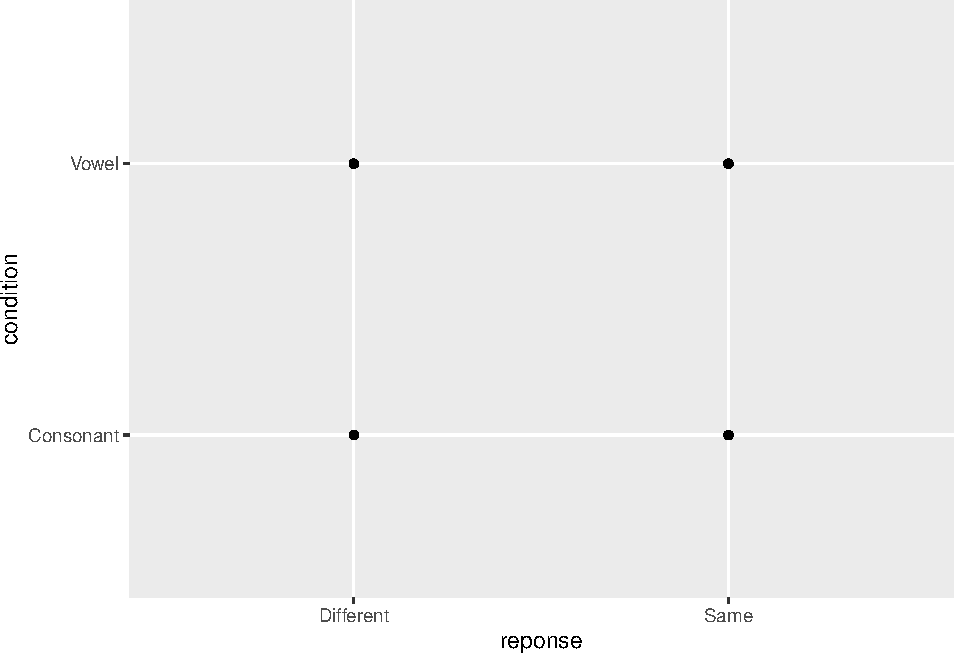
\includegraphics{analysis_files/figure-latex/e2-1-1.pdf}

\subsubsection{Exercise 2.2}\label{exercise-2.2}

\begin{Shaded}
\begin{Highlighting}[]
\NormalTok{data\_e2\_2 }\OtherTok{\textless{}{-}} \FunctionTok{read\_csv}\NormalTok{(}\StringTok{"data/data\_e2\_2.csv"}\NormalTok{)}
\end{Highlighting}
\end{Shaded}

\begin{verbatim}
## Rows: 1035 Columns: 2
## -- Column specification --------------------------------------------------------
## Delimiter: ","
## chr (1): voicing
## dbl (1): vot
## 
## i Use `spec()` to retrieve the full column specification for this data.
## i Specify the column types or set `show_col_types = FALSE` to quiet this message.
\end{verbatim}

\begin{Shaded}
\begin{Highlighting}[]
\NormalTok{data\_e2\_2 }\SpecialCharTok{\%\textgreater{}\%}
  \FunctionTok{ggplot}\NormalTok{(}\FunctionTok{aes}\NormalTok{(vot, }\AttributeTok{fill =}\NormalTok{ voicing)) }\SpecialCharTok{+}
  \FunctionTok{geom\_bar}\NormalTok{(}\AttributeTok{width=}\FloatTok{0.5}\NormalTok{)}
\end{Highlighting}
\end{Shaded}

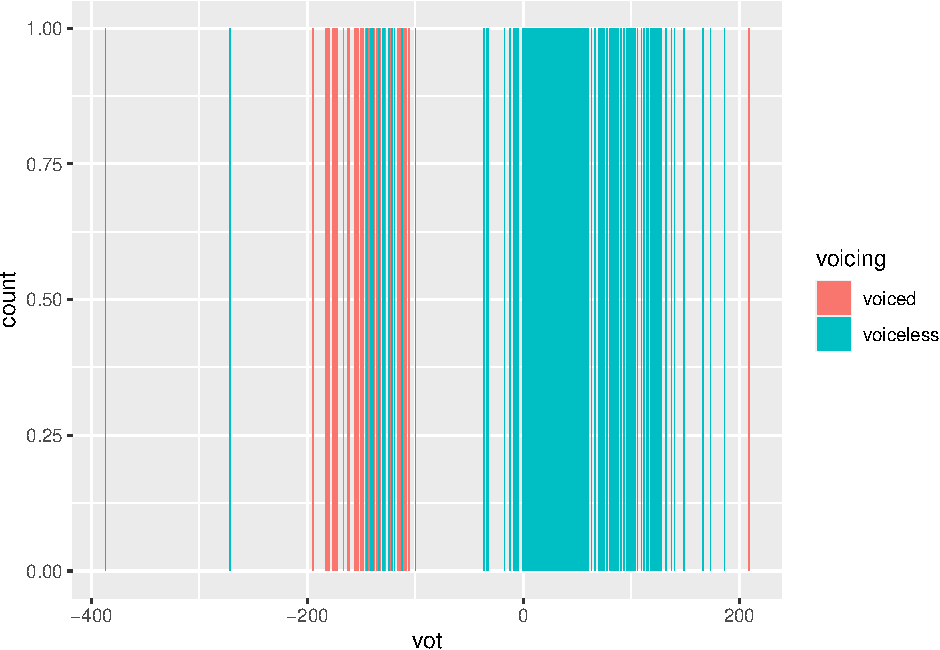
\includegraphics{analysis_files/figure-latex/e2-2-1.pdf}

\newpage

\subsection{Exercise 3: Choosing appropriate summary
measures}\label{exercise-3-choosing-appropriate-summary-measures}

Read in \texttt{data\_e3.csv} and obtain summary measures (central
tendency: mean, median, or mode; dispersion: standard deviation or
range) for each variable in the data. Make sure to pick the correct
measure(s) for the respective variable type.

Then, for each variable, briefly state the type of variable, the chosen
measure(s), and report the value of the measure(s).

\newpage

\subsection{Exercise 4: Identifying probability
distributions}\label{exercise-4-identifying-probability-distributions}

For each variable in the table below, specify in the ``Probability
distribution'' column whether it's (in principle) distributed according
to a Gaussian, a log-normal, or a Bernoulli distribution, or according
to some different one (put ``other'' in this case).

If you have doubts about any of the variables, you can write about it
briefly below the table.

\begin{longtable}[]{@{}lll@{}}
\toprule\noalign{}
& Variable & Probability distribution \\
\midrule\noalign{}
\endhead
\bottomrule\noalign{}
\endlastfoot
1 & Vowel duration (ms) & \\
2 & Formant values (hz) & \\
3 & Accuracy (binary) & \\
4 & Readability (0-100) & \\
5 & Reaction times (ms) & \\
6 & Number of relative clauses & \\
7 & Scots vs English & \\
8 & Counts of infant gestures & \\
9 & Logged reaction times & \\
10 & Ratio of 1st vs non-1st pronouns & \\
\end{longtable}

\newpage

\subsection{Exercise 5: Running a Bayesian linear
model}\label{exercise-5-running-a-bayesian-linear-model}

\end{document}
